\documentclass[a4paper]{article}
\usepackage{geometry}
\usepackage{multicol}
\usepackage{setspace}
\usepackage{listings}
\usepackage{graphicx}
\usepackage{algorithm}
\usepackage{algpseudocode}
\usepackage{amsmath}
\usepackage{amssymb}
\usepackage{multicol}
\usepackage{float}
\DeclareGraphicsExtensions{.eps,.ps,.jpg,.bmp}
\usepackage{xcolor}
%\setlength{\parskip}{0.5\baselineskip}
\geometry{left=3.0cm,right=2.0cm,top=1.5cm,bottom=2.0cm} 
\title{\textbf{Algorithmn HW8}}
\author{5140379032 JIN YI FAN}
\date{}
\begin{document}
\maketitle
\begin{spacing}{1.3}
%\begin{multicols}{2}
\section*{Problem 8.5}
\begin{algorithmic}[1]
\Require total value of money to pay $n<2^{k+1}$
\Ensure combination plan $plan[0\ldots k]=\{c_0\ldots c_k\}$, $c_i$ refers to number of coin values $2^i$
\State $plan[0\ldots k]\gets 0$
\For{$i\gets k$ to $0$}
\State $plan[i]\gets \lfloor n/(2^i)\rfloor$
\State $n\gets (n-plan[i]*2^k)$
\EndFor
\State \textbf{return} $plan$
\end{algorithmic}

\begin{multicols}{2}
\section*{Problem 8.7}
\begin{multicols}{2}
\begin{figure}[H]
    \centering
    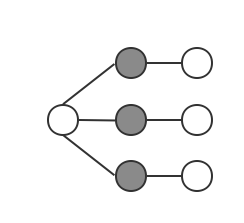
\includegraphics[width=3.5cm]{vertex.png}
\end{figure}
If we take the introduced greedy approach, 
we may get the vertex cover as all the 4 white vertexes.
But actually it should be the set of 3 grey vertexes.
\end{multicols}

\section*{Problem 8.8}
\begin{multicols}{2}
\begin{figure}[H]
    \centering
    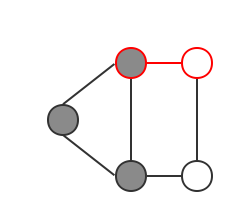
\includegraphics[width=3.5cm]{clique.png}
\end{figure}
If we take the introduced greedy approach,
very likely we will delete the left single vertex and get 
the red clique, but actually the grey clique is the required one. 
\end{multicols}
\end{multicols}

\section*{Problem 8.27}
\textbf{Yes}.
\\Because actually we can add a big enough constant to all the weights of edges to make sure each weight is a positive number. MST of this graph won't change.

\section*{Problem 8.28}
\textbf{Assumptions:} $T_1$, $T_2$ are two minimum spanning trees of $G(V,E)$, 
and $T_1.E=(a_1,a_2\ldots a_k\ldots a_n)$, $T_2.E=(b_1,b_2\ldots b_k\ldots b_n)$
, both ordered by weight in ascending order and $k$ is the minimum subscript s.t. 
$weight(a_k)\neq weight(b_k)$, thus $a_k \no tin T_2.E$ and $b_k \notin T_1.E$.
\\We can assume that $weight(a_k) < weight(b_k)$ in this case.
\\Then $T_2\cup a_k$ must contain a cycle $C$.
\\$\because$ $\forall i<k,a_i=b_i$, and $\{a_1\ldots a_{k-1},a_{k}\}$ shouldn't become cycle,
\\$\therefore$ $\{b_1\ldots b_{k-1},a_{k}\}$ won't become a cycle,
\\$\therefore$ $\exists b_j\in C,\ s.t.\ weight(b_j)>weight(a_k)$,
\\$\therefore$ $T_2$ shouldn't be a minimum spanning tree of $G$, which leads to a contradiction.

\section*{Maximum Spanning Tree}
\begin{algorithmic}[1]
\Require A weighted graph $G=(V,E)$
\Ensure The maximum spanning tree $T=(V_M,E_M)$
\State $sum\gets \sum\limits_{e_i\in E}weight(e_i)$
\For{each $e\in E$}\Comment{reverse the weights of the edges in $E$}
\State append $(u,v,(sum-weight(e)))$ to $E_r$ 
\EndFor
\State $(V_M,E_M)\gets$ \Call{Prim}{$V,E_r$}\Comment{do Prim}
\For{each $e\in E_M$}\Comment{recover the weights of the edges in $E_M$}
\State $weight(e)\gets (sum-weight(e))$
\EndFor
\State \textbf{return} $(V_M,E_M)$
\end{algorithmic}

%\end{multicols}
\end{spacing}
\end{document}

